\documentclass[main.tex]{subfiles}
\begin{document}

\chapter{Spring}
\section{Spring AOP}
\subsection{描述一下Spring AOP及关注点和横切关注点}
AOP即面向切面编程,剖解开封装的对象内部,并将那些影响了多个类的公共行为封装到一个可重用模块,并将其名为“Aspect”,即切面。简单地说,就是将那些与业务无关,却为业务模块所共同调用的逻辑封装起来,便于减少系统的重复代码,降低模块间的耦合度,并有利于未来的可操作性和可维护性。Spring中AOP代理由Spring的IOC容器负责生成、管理,其依赖关系也由IOC容器负责管理。因此,AOP代理可以直接使用容器中的其它bean实例作为目标,这种关系可由IOC容器的依赖注入提供。AOP的关键单元是切面,或者说关注点,即为我们想实现特定业务功能的方法。一些切面可能有集中的代码,但是有些可能被分散或者混杂在一起,例如日志或者事务。这些分散的切面被称为横切关注点。横切关注点是贯穿整个应用程序的关注点。像日志、安全和数据转换。\\
AOP的最大意义其实就是在不改变原来代码的前提下,也不对源代码做任何协议接口要求。而实现了类似插件的方式,来修改源代码,给源代码插入新的执行代码。
\subsection{Spring中有哪些不同的通知类型}
通知(advice)是切面的具体逻辑实现。有以下5种形式:
\begin{enumerate}
    \item 前置通知(Before Advice):在连接点之前执行的Advice,不过除非它抛出异常,否则没有能力中断执行流。使用@Before注解使用这个Advice。
    \item 返回后通知(After Retuning Advice):在连接点正常结束之后执行的Advice。例如一个方法没有抛出异常并正常返回。通过@AfterReturning注解来使用。
    \item 抛出(异常)后执行通知(After Throwing Advice):如果一个方法通过抛出异常来退出的话,这个Advice就会被执行。通过@AfterThrowing注解来使用。
    \item 后置通知(After Advice):无论连接点是通过什么方式退出的(正常返回或者抛出异常)都会执行在结束后执行这些Advice。通过@After注解使用。
    \item 环绕通知(Around Advice):决定是否调用目标方法,而且能够获得到目标方法的返回值,而且还能改变这些返回值。通过@Around注解使用。
\end{enumerate}
\subsection{代理模式}
代理模式给某一个对象提供一个代理对象,并由代理对象控制对原对象的引用。其主要特点是在不改变原有类的前提下,在原有类某些方法执行前后,插入执行任意代码。所以代理模式需要写新的类对原有的类进行包装,有如下三种实现方式:
\subsubsection{静态代理}
需要增强原有类的哪个方法,就需要对在代理类中包装哪个方法。在使用时,需要定义接口或者父类,被代理对象与代理对象一起实现相同的接口或者是继承相同父类。例如:\\
接口IUserDao.java
\begin{minted}{java}
    public interface IUserDao {
        void save();
    }
\end{minted}
需要代理的目标对象UserDao.java
\begin{minted}{java}
    public class UserDao implements IUserDao {
        public void save() {
            System.out.println("---- Already saved!----");
        }
    }
\end{minted}
代理对象UserDaoProxy.java
\begin{minted}{java}
    public class UserDaoProxy implements IUserDao {
        // the object needed to be proxied
        private IUserDao target;

        public UserDaoProxy(IUserDao target){
            this.target=target;
        }

        public void save() {
            System.out.println("Start transaction");
            target.save(); // the target method
            System.out.println("Commit transaction");
        }
    }
\end{minted}
测试类App.java
\begin{minted}{java}
    public class App {
        public static void main(String[] args) {
            UserDao target = new UserDao();
            // proxy object
            UserDaoProxy proxy = new UserDaoProxy(target);
            proxy.save();
        }
    }
\end{minted}
静态代理的缺点是代理对象需要与目标对象实现一样的接口,所以会产生很多代理类,为日后的维护增添麻烦。
\subsubsection{动态代理}
动态代理利用反射机制,对象和方法都是传入的变量,以此动态调用被代理对象的任何方法,JDK实现代理,只需要使用newProxyInstance方法,还是上面的那个例子,只不过我们这次用动态代理机制来将其实现一下:\\
代理工厂类ProxyFactory.java
\begin{minted}{java}
    public class ProxyFactory {
        // the object which needed to be proxied
        private Object target;

        public ProxyFactory(Object target){
            this.target=target;
        }

        // generate proxy instance
        public Object getProxyInstance(){
            // invoke newProxyInstance method
            return Proxy.newProxyInstance(
                    target.getClass().getClassLoader(),
                    target.getClass().getInterfaces(),
                    new InvocationHandler() {
                        @Override
                        public Object invoke(Object proxy, Method method, Object[] args) throws Throwable {
                            System.out.println("Start transaction");
                            // invoke target object method and get return value
                            Object returnValue = method.invoke(target, args);
                            System.out.println("Commit transaction");
                            return returnValue;
                        }
                    }
            );
        }
    }
\end{minted}
测试类App.java
\begin{minted}{java}
    public class App {
        public static void main(String[] args) {
            // original object
            IUserDao target = new UserDao();
            System.out.println(target.getClass());

            // get a proxy instance for target object
            IUserDao proxy = (IUserDao) new ProxyFactory(target).getProxyInstance();
            System.out.println(proxy.getClass());

            // invoke method
            proxy.save();
        }
    }
\end{minted}
\subsubsection{CGLIB代理}
静态代理和动态代理都要求目标对象是实现一个特定接口的目标对象,但有的时候一个对象是一个单独的对象,并没有实现任何接口,这个时候就可以使用以目标对象子类的方式类实现代理,即CGLIB代理,也叫做子类代理。显然,代理的类不能被标记为final,否则报错。\\
使用CGLIB代理时需要引入cglib的jar文件,如果你用了Spring,其核心中已经包括了这个包,所以可以直接引入包spring-core,代码实例:\\
没有实现任何接口的目标对象类UserDao.java
\begin{minted}{java}
    public class UserDao {
        public void save() {
            System.out.println("----已经保存数据!----");
        }
    }
\end{minted}
CGLIB代理工厂ProxyFactory.java
\begin{minted}{java}
    public class ProxyFactory implements MethodInterceptor {
        // the target object needed to be proxied
        private Object target;

        public ProxyFactory(Object target) {
            this.target = target;
        }

        // create a proxy object instance
        public Object getProxyInstance(){
            // tool instance
            Enhancer en = new Enhancer();
            // set super class of CGLIB proxy
            en.setSuperclass(target.getClass());
            en.setCallback(this);
            // create proxy instance
            return en.create();
        }

        @Override
        public Object intercept(Object obj, Method method, Object[] args, MethodProxy proxy) throws Throwable {
            System.out.println("Start transaction");
            // invoke the super class method
            Object returnValue = method.invoke(target, args);
            System.out.println("Commit transaction");
            return returnValue;
        }
    }
\end{minted}
测试类App.java
\begin{minted}{java}
    public class App {
        @Test
        public void test(){
            UserDao target = new UserDao();
            UserDao proxy = (UserDao) new ProxyFactory(target).getProxyInstance();
            proxy.save();
        }
    }
\end{minted}

\section{Spring IOC}
\subsection{IOC的基本思想}
IOC即Inversion of Control,控制反转。通常,每个对象在使用他的合作对象时,自己需要使用像new Object()这样的语句来完成合作对象的申请工作。这样会造成对象间的耦合度高。IOC的思想是:Spring容器来实现这些相互依赖对象的创建、协调工作。对象只需要关系业务逻辑本身就可以了。从这方面来说,对象如何得到他的协作对象的责任被反转了(IOC、DI)。\\
Spring所倡导的开发方式就是如此:所有的类都会在spring容器中登记,告诉spring你是个什么东西,你需要什么东西,然后spring会在系统运行到适当的时候,把你要的东西主动给你,同时也把你交给其他需要你的东西。所有的类的创建、销毁都由spring来控制,也就是说控制对象生存周期的不再是引用它的对象,而是spring。对于某个具体的对象而言,以前是它控制其他对象,现在是所有对象都被spring控制,所以这叫控制反转。
\subsection{依赖注入DI}
IoC的一个任务是在系统运行中,动态的向某个对象提供它所需要的其他对象。这一点是通过DI(Dependency Injection,依赖注入)来实现的。比如对象A需要操作数据库,以前我们总是要在A中自己编写代码来获得一个Connection对象,有了 spring我们就只需要告诉spring,A中需要一个Connection,至于这个Connection怎么构造,何时构造,A不需要知道。A需要依赖Connection才能正常运行,而这个Connection是由spring注入到A中的,这即为依赖注入。

\section{Spring Bean}
\subsection{bean的作用域}
bean一共有如下5种作用域:
\begin{enumerate}
    \item singleton(单例):在IoC容器中仅存在一个bean实例,以单例的形式存在,默认值。
    \item prototype(原型):每次请求都会创建一个新的bean实例,即每次调用getBean()时,相当于执行new XXBean()。
    \item request:每次HTTP请求都会创建一个新的bean,该bean仅在当前HTTP request内有效,该作用域仅适用于WebApplicationContext环境。
    \item session:每一次HTTP请求都会产生一个新的bean,该bean仅在当前HTTP session内有效,仅适用于WebApplicationContext环境。
    \item global-session:所有的session共享一个bean实例
\end{enumerate}
设置bean的作用域:\\
\begin{minted}{xml}
    <bean id="..." class="..." scope="singleton">
        ...
    </bean>
\end{minted}
在xml中我们可以使用属性lazy-init=“true”来延迟加载bean,这样,只有在第一次获取bean时,才会初始化bean,或者使用注解的形式:\\
\begin{minted}{java}
    @Service
    @Scope("singleton")
    public class ServiceImpl{

    }
\end{minted}

\subsection{bean的加载}
\begin{figure}[H]
    \centering
    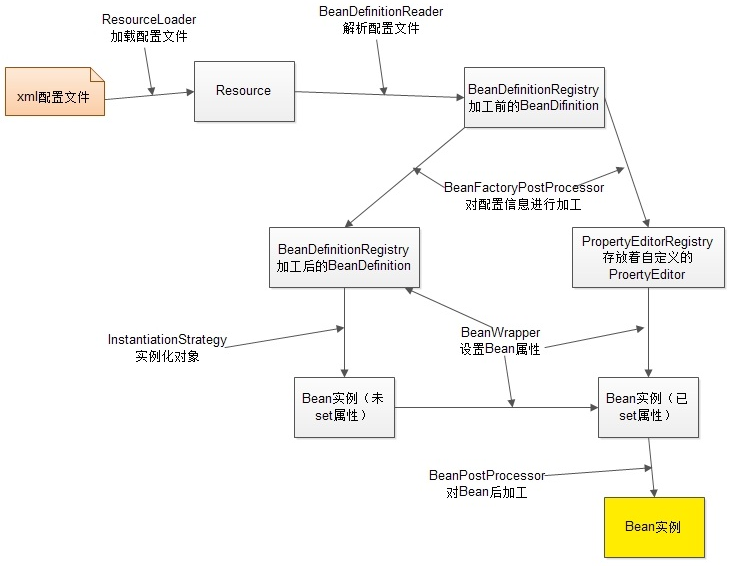
\includegraphics[scale=0.75]{./images/0018.png}
    \caption{bean的加载流程}
\end{figure}
\begin{enumerate}
    \item ResourceLoader从XML中加载Spring配置信息,并使用Resource表示这个配置文件的资源。
    \item BeanDefinitionReader读取Resource所指向的配置文件资源,然后解析配置文件。配置文件中每一个<bean>解析成一个BeanDefinition对象,并保存到BeanDefinitionRegistry中。
    \item 容器扫描BeanDefinitionRegistry中的BeanDefinition,使用Java的反射机制自动识别出实现了Bean工厂后处理器接口(BeanFactoryPostProcessor)的Bean,然后调用这些Bean工厂后处理器对BeanDefinitionRegistry中的BeanDefinition进行加工处理。在此过程中主要完成如下两项工作:
        \begin{enumerate}
            \item 对使用占位符<bean>的标签进行解析得到最终的配置值
            \item 对BeanDefinitionRegistry中的BeanDefinition进行扫描,通过反射机制找出所有实现了java.beans.PropertyEditor接口的Bean,然后将其注册到Spring容器的属性编辑器注册表中(PropertyEditorRegistry)。
        \end{enumerate}
    \item Spring容器从BeanDefinitionRegistry中取出加工后的BeanDefinition,并调用InstantiationStrategy着手进行Bean实例化的工作。
    \item 在实例化Bean时,Spring容器使用BeanWrapper对Bean进行封装,BeanWrapper通过反射机制操作Bean中的方法,结合该Bean的BeanDefinition以及容器中属性编辑器,完成Bean属性的设置工作。
    \item 利用容器中注册的Bean后处理器(实现BeanPostProcessor接口的Bean)对已经完成属性设置工作的Bean进行后续加工,直接装配出一个准备就绪的Bean。
\end{enumerate}

\section{Spring MVC}
\subsection{Spring MVC的工作流程}
客户端发送请求 -> 前端控制器DispatcherServlet接受客户端请求 -> 找到处理器映射HandlerMapping解析请求对应的Handler -> HandlerAdapter会根据Handler来调用真正的处理器开始处理请求,并处理相应的业务逻辑 -> 处理器返回一个模型视图ModelAndView -> 视图解析器进行解析 -> 返回一个视图对象 -> 前端控制器DispatcherServlet渲染数据(Moder) -> 将得到视图对象返回给用户。
\begin{figure}[H]
    \centering
    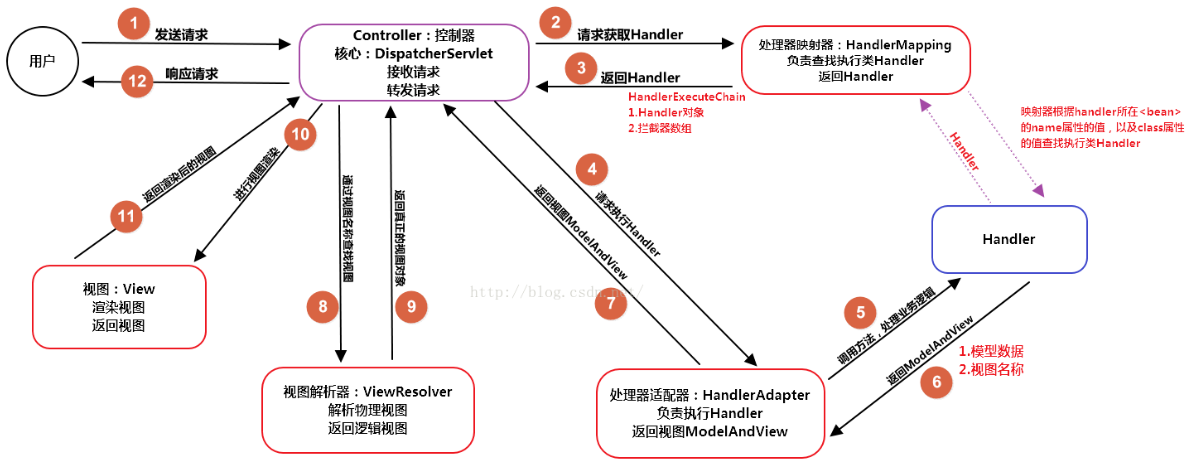
\includegraphics[scale=0.65]{./images/0016.png}
    \caption{Spring MVC工作流程}
\end{figure}
\subsection{SpringMVC怎么样设定重定向和转发的}
在返回值前面加"forward:"就可以让结果转发,譬如"forward:user.do?name=method4"\\
在返回值前面加"redirect:"就可以让返回值重定向,譬如"redirect:http://www.baidu.com"。

\end{document}
